\section{Whole trajectories under the original engine}
\label{sec:traj}

Counterfactual replay judges single decisions. Agents may give themselves away more clearly in \emph{how} they shop: how many products they compare, whether they go back, how they search. We test this on WebShop, the one setting where both classes can produce complete sessions in the same environment.

\paragraph{Setup.} We rebuilt WebShop's original search engine (pyserini 0.17 BM25 over the full catalog of 1.18M products). For 99.6\% of 2{,}364 human searches it reproduces the logged first results page exactly, so the engine confound of \S\ref{sec:pilot} is removed. Claude Haiku 5.5 and DeepSeek V4 Flash then shopped in the official WebShop text environment. They had the humans' action space (search, paginate, open product, choose options, read sub-pages, buy) and up to 20 steps per episode. Their goals were the same 150 instructions as the test humans, with each human's target product and price limit. This gives 150 human--agent pairs per model.

We compute 14 trajectory features with one function for both classes:
\begin{itemize}
  \item pages visited, queries and reformulations, query length and overlap with the instruction;
  \item products viewed, deepest results page, sub-pages, option clicks, returns to the results list;
  \item purchase, and the rank of the purchased item.
\end{itemize}
\bgpt{} scores each session with the vendor method: mean excess surprisal, its $z$-score, mean log-rank, and one-sided CUSUM statistics in both directions (``surprising'' and ``too normal''). Calibration uses human sessions from the other fold. Detectors use 5-fold cross-validation grouped by instruction pair.

\begin{figure}[t]
\centering
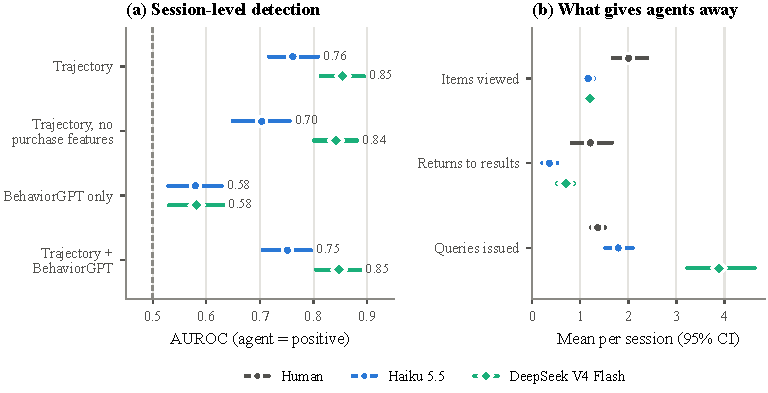
\includegraphics[width=\linewidth]{figures/fig_traj.pdf}
\caption{\textbf{Whole trajectories, same engine.} (a) Session-level AUROC with 95\% pair-bootstrap intervals. Trajectory features detect both agents. The control without purchase features addresses the fact that every human demonstration ends in a purchase. \bgpt{} alone stays near 0.58 and adds nothing when combined. (b) Haiku compares few products and rarely goes back to the results; DeepSeek over-searches.}
\label{fig:traj}
\end{figure}

\paragraph{Results.} Trajectory features separate humans from agents well: AUROC 0.76 [0.72, 0.81] for Haiku and 0.85 [0.81, 0.89] for DeepSeek (Fig.~\ref{fig:traj}a). Every human demonstration ends in a purchase, whereas agents sometimes stop without buying. To rule this out as the source of the signal, we dropped the purchase-related features (0.70 and 0.84) and also kept only pairs in which the agent bought (0.66 and 0.81). Both checks leave the trajectory detector well above \bgpt{}, which reaches 0.58 for both agents on its own and lowers the combined detector slightly (by 0.01 for both agents).

The two agents are caught in different ways (Fig.~\ref{fig:traj}b). Haiku hardly comparison-shops: it views 1.2 products per session against 2.0 for humans and returns to the results list 0.35 times against 1.2. DeepSeek over-searches, issuing 3.9 queries per session against 1.4 for humans, and shorter ones (5.8 vs.\ 6.7 words). On the \bgpt{} side, agent sessions are again slightly \emph{less} surprising than human ones (mean excess surprisal 0.02 for Haiku and 0.08 for DeepSeek, against 0.10 for humans), but the difference does not separate the classes.

\paragraph{Why the foundation model misses it.} \bgpt{} scores \emph{which product} is chosen next. A WebShop session yields a median of one scored step, and the behaviors that separate the classes (comparing, backtracking, reformulating) are navigation, which a next-item model does not score. Timing could add further signal, but the model ignores time below the hour.
